\documentclass[a4paper]{article}
\usepackage[english]{babel}
\usepackage[utf8x]{inputenc}
\usepackage[T1]{fontenc}
\usepackage[left=3.0cm, right=2.0cm, top=2.5cm, bottom=2.5cm]{geometry}
\usepackage{amsmath}
\usepackage{graphicx}
\usepackage{caption}
\usepackage{float}

\date{}

\begin{document}
\newpage
\thispagestyle{empty}


\begin{center}
\centering

\includegraphics[keepaspectratio,scale=2]{WUT_logo.jpeg} \\[1.0cm]
{\fontsize{17}{17}\selectfont
\textsc{Warsaw University of Technology \\[1.5cm]
Faculty of Power and Aeronautical Engineering  \\[.5cm]
Institute of Heat Engineering  \\[1.0cm]}
\huge{Aerospace Engineering \\[1.7cm]}}
\fontsize{30}{30}\selectfont
\textbf{Autoignition of methane-air mixture \\[3.0cm]}
\huge{Agata Łuczak \\ 271302}
\end{center}

\newpage


\begin{abstract}
    The purpose of this project was an analysis of the role and the impact of initial temperature, pressure and equivalence ratio in a process of autoignition of methane-air mixture. The simulation was set up using Cantera in Python and the results of performed calculations were saved in a data file, but also depicted as plots.
\end{abstract}
\section{Introduction and mathematical model}
Autoignition refers to a homogenous ignition of the fuel-oxidizer mixture. Homogenous means there is no external ignition source needed. The autoignition temperature is defined as the limit temperature above which  mixture ignites given enough time. When it comes to autoignition temperature and time form a pair of values which are mutually dependent. The autoignition time is much more relevant, because it can be directly compared to the residence time in the premixing section of gas turbine combustors.\\\\
Methane-air mixture's simulation was conducted under specific conditions in a closed reactor for $10$ various temperatures, pressures, equivalence ratios. The moment of the sharpest temperature increase is the autoignition point and to be able to catch that exact point time step was set to $10^{-6}$ and number of iterations to $10^5$.
\subsection{Stoichiometry}
\begin{center}
    $CH_4 +2(0_2+3,76N_2)=CO_2+2H_2O$\\
    \bigskip
   (F/A)$_{stoichiometric}$ = \( \frac{1}{2(1+3,76)} \) = $0,105042$\\
   \bigskip
   $\phi =  \frac{F/A}{(F/A)_{stoichiometric}}$\\
   \bigskip
   F/A = $\phi*(F/A)_{stoichiometric}$\\
   \bigskip
   A = $\frac{F}{\phi*(F/A)_{stoichiometric}}$
\end{center}
Assuming constant number of methane moles, only the number of air moles would change accordingly to the equation above.     
\subsection{Boundary conditions}
\begin{center}
    $P_{min} = 101325 Pa$\\
    \bigskip
    $P_{max} = 303975 Pa$\\
    \bigskip
    $T_{min} = 1300 K$\\
    \bigskip
    $T_{max}= 2500 K$\\
    \bigskip
    $\phi_{min} = 0.4$\\
    \bigskip
    $\phi_{max} = 3.1$\\
\end{center}
\newpage
\section{Results}
Acquired through simulation data was successfully imported to .csv file and plots are shown below.

\begin{figure}[H]
\centering
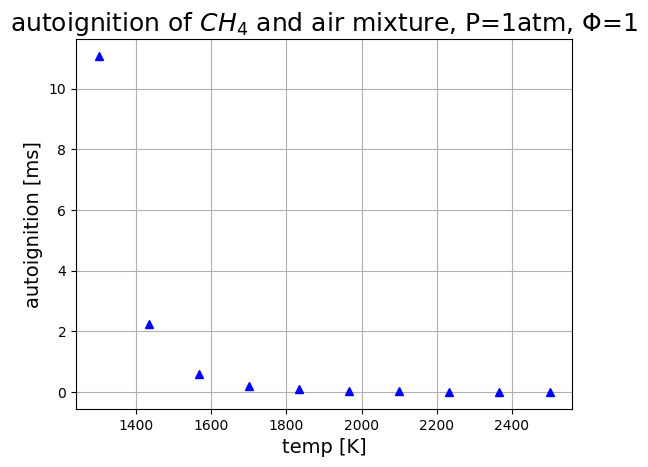
\includegraphics[width=0.8\textwidth]{autoignition_initialtemperature.png}
\caption{Autoignition time as a function of initial temperature}
\end{figure}
The autoignition time decreases expotentially and very drastically with increasing unburned mixture temperature, however, after some point around 1700K onwards the differences between autoignition times aren't very significant, it's more stable.In this project minimal initial temperature was set to 1300K, but considering the trend for lower temperatures autoignition probably doesn't occur at all.

\begin{figure}[H]
\centering
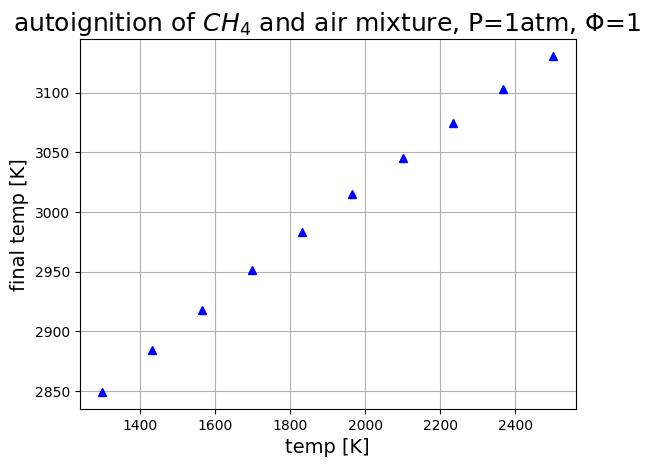
\includegraphics[width=0.8\textwidth]{finaltemp_temp.png}
\caption{Final temperature as a function of initial temperature}
\end{figure}
\newpage
The final temperature increases almost linearly with initial temperature's increase.

\begin{figure}[H]
\centering
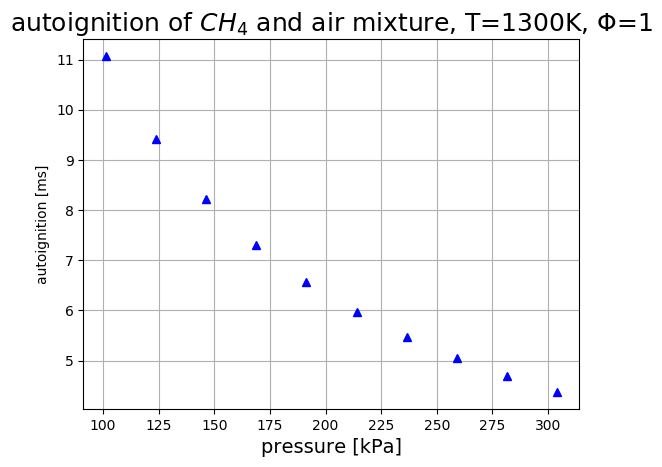
\includegraphics[width=0.8\textwidth]{autoignition_pressure.png}
\caption{Autoignition time as a function of pressure}
\end{figure}
Autoignition time decreases as pressure's values are higher. The bigger pressure the smaller function's gradient.

\begin{figure}[H]
\centering
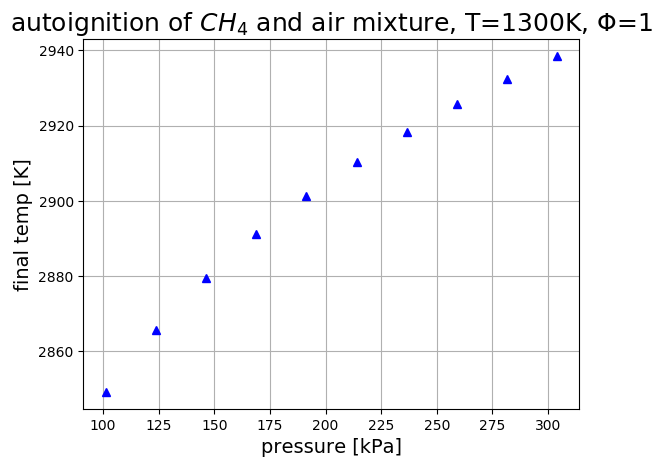
\includegraphics[width=0.8\textwidth]{finaltemp_pressure.png}
\caption{Final temperature as a function of pressure}
\end{figure}
The value of final temperature rises for greater pressures, however, even after tripling the pressure, temperature's increase isn't as rapid.

\begin{figure}[H]
\centering
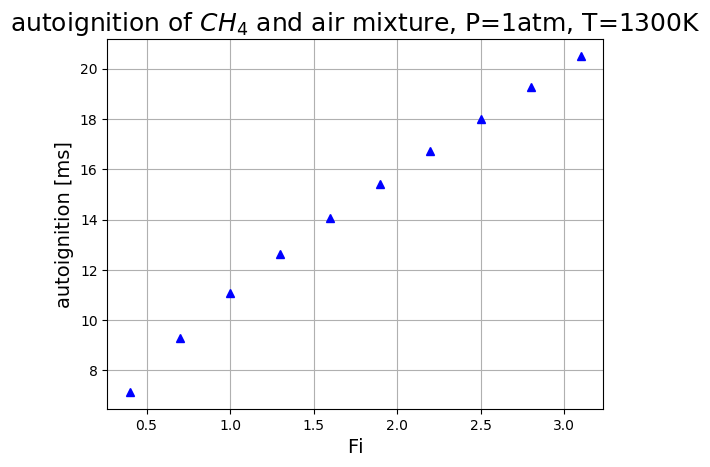
\includegraphics[width=0.8\textwidth]{autoignition_Fi.png}
\caption{Autoignition time as a function of equivalence ratio}
\end{figure}
Increasing equivalence ratio causes growth of the autoignition time.

\begin{figure}[H]
\centering
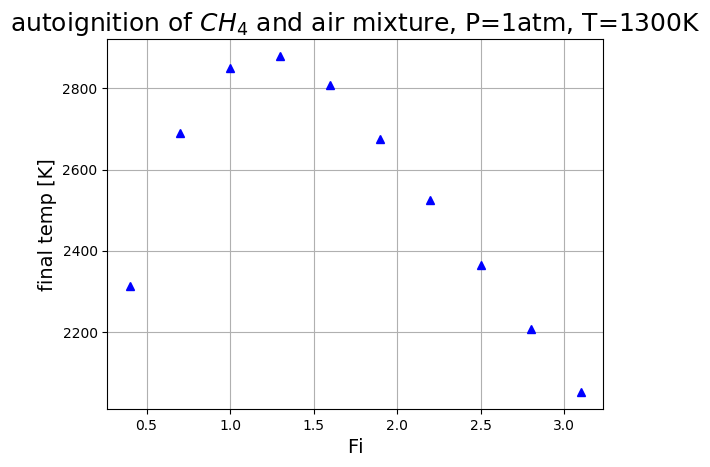
\includegraphics[width=0.8\textwidth]{finaltemp_Fi.png}
\caption{Final temperature as a function equivalence ratio}
\end{figure}
The greatest value of final temperature is reached for $\phi$ around 1.3 as it appears to be the most favourable value of the coefficient. Equivalence ratio has seemingly the biggest influence on the final temperature's characteristics, thus it's a crucial parameter in the autoignition process.
\section{Conclusion}
Conducted study proves that autoignition of methane-air mixture is highly dependant on fundamental parameters such as temperature, pressure and $\phi$.\\
Simulations of autoignition processes can be useful in a variety of fields, for example autoignition temperatures are vitally important for process designs as it is the temperature to prevent or eliminate readily available ignition sources, which is specified for some plant equipment, e.g., operating temperatures of electrical equipment, lighting fixtures, etc.

\begin{thebibliography}{9}
\bibitem{1}
\textit{CANTERA\textunderscore HandsOn.pdf}
\bibitem{2} 
\texttt{https://www.sciencedirect.com/topics/engineering/autoignition}
\end{thebibliography}

\end{document}


